\documentclass{standalone}
\usepackage{tikz}
\usepackage{nono}
\begin{document}
\begin{tikzpicture} 
  \fill[gray!20] (-0.5, 4) circle (2cm);
  \draw[thick] (3,1) -- (3, 4) coordinate (O) -- (5, 4) coordinate (A);
  \draw (5,4) -- (4.5, 2) -- (5.5, 2) --cycle;
  \draw[fill=gray] (4.8, 2) rectangle (5.2, 2.3);
  \draw (6,0) node[above right]{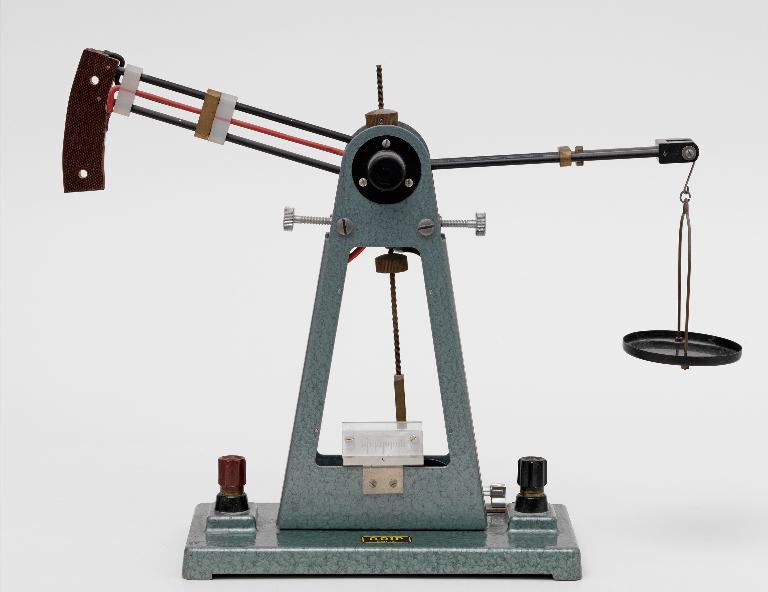
\includegraphics[height=7cm]{images/balance_cotton.jpg}};
  \draw (O) -- ++(135:4) arc(135:180:4) -- ++(1, 0) arc(180:135:2.9) -- ++(-45:3);
  \draw [fill=white] (O) circle (3pt) node[below right=3pt]{$O$} ;
  \draw (5, 2) node[below]{$m$}; 
  \draw[-latex] (-0.5, 4) -- ++(0.1, 0) node[midway, below right]{$i$}; 
  \draw[dashed] (O) -- ++(0,1) coordinate(B); 
  \draw[dashed] (A) -- ++(0,1) coordinate(C); 
  \draw[<->] (B) -- (C) node[midway, below] {$a$}; 
  \draw[dashed] (-0.5, 4) -- ++(0, -1) coordinate (D);
  \draw[<->] (D) -- (3, 3) node[midway, below]{$a'$} ;
  \fill (-1.5, 3.5) circle(1pt);
  \draw (-1.5, 3.5) circle(5pt) node[below=5pt]{$\vv{B}$} ;
  \draw[dashed] (0, 4) -- ++(0, 1) coordinate(A);
  \draw[dashed] (-1, 4) -- ++(0, 1) coordinate (B);
  \draw[<->] (A) -- (B) node[midway, above] {$L$}; 
\end{tikzpicture}
\end{document}
